%%%%%%%%%%%%%%%%%%%%%%%%%%%%%%%%%%%%%%%%%
% Jacobs Portrait Poster
% LaTeX Template
% Version 1.0 (31/08/2015)
% (Based on Version 1.0 (29/03/13) of the landscape template
%
% Created by:
% Computational Physics and Biophysics Group, Jacobs University
% https://teamwork.jacobs-university.de:8443/confluence/display/CoPandBiG/LaTeX+Poster
% 
% Further modified by:
% Nathaniel Johnston (nathaniel@njohnston.ca)
%
% Portrait version by:
% John Hammersley
%
% The landscape version of this template was downloaded from:
% http://www.LaTeXTemplates.com
%
% License:
% CC BY-NC-SA 3.0 (http://creativecommons.org/licenses/by-nc-sa/3.0/)
%
%%%%%%%%%%%%%%%%%%%%%%%%%%%%%%%%%%%%%%%%%

%----------------------------------------------------------------------------------------
%	PACKAGES AND OTHER DOCUMENT CONFIGURATIONS
%----------------------------------------------------------------------------------------

\documentclass[final]{beamer}

\usepackage[scale=1.24]{beamerposter} % Use the beamerposter package for laying out the poster

\usetheme{confposter} % Use the confposter theme supplied with this template

\setbeamercolor{block title}{fg=ngreen,bg=white} % Colors of the block titles
\setbeamercolor{block body}{fg=black,bg=white} % Colors of the body of blocks
\setbeamercolor{block alerted title}{fg=white,bg=dblue!70} % Colors of the highlighted block titles
\setbeamercolor{block alerted body}{fg=black,bg=dblue!10} % Colors of the body of highlighted blocks
% Many more colors are available for use in beamerthemeconfposter.sty

%-----------------------------------------------------------
% Define the column widths and overall poster size
% To set effective sepwid, onecolwid and twocolwid values, first choose how many columns you want and how much separation you want between columns
% In this template, the separation width chosen is 0.024 of the paper width and a 4-column layout
% onecolwid should therefore be (1-(# of columns+1)*sepwid)/# of columns e.g. (1-(4+1)*0.024)/4 = 0.22
% Set twocolwid to be (2*onecolwid)+sepwid = 0.464
% Set threecolwid to be (3*onecolwid)+2*sepwid = 0.708

\newlength{\sepwid}
\newlength{\onecolwid}
\newlength{\twocolwid}
\newlength{\threecolwid}
\setlength{\paperwidth}{36in} % A0 width: 46.8in
\setlength{\paperheight}{48in} % A0 height: 33.1in
\setlength{\sepwid}{0.024\paperwidth} % Separation width (white space) between columns
\setlength{\onecolwid}{0.22\paperwidth} % Width of one column
\setlength{\twocolwid}{0.464\paperwidth} % Width of two columns
\setlength{\threecolwid}{0.708\paperwidth} % Width of three columns
\setlength{\topmargin}{-0.5in} % Reduce the top margin size
%-----------------------------------------------------------

\usepackage{graphicx}  % Required for including images

\usepackage{booktabs} % Top and bottom rules for tables

%----------------------------------------------------------------------------------------
%	TITLE SECTION 
%----------------------------------------------------------------------------------------

\title{The Testing/Characterization of interfaces and Molecular Simulation in Lithium-ion batteries} % Poster title

\author{Feiyu Xiao} % Author(s)

\institute{TEEP 4, School of Aerospace Engineering} % Institution(s)

%----------------------------------------------------------------------------------------

\begin{document}

\addtobeamertemplate{block end}{}{\vspace*{2ex}} % White space under blocks
\addtobeamertemplate{block alerted end}{}{\vspace*{2ex}} % White space under highlighted (alert) blocks

\setlength{\belowcaptionskip}{2ex} % White space under figures
\setlength\belowdisplayshortskip{2ex} % White space under equations

\begin{frame}[t] % The whole poster is enclosed in one beamer frame

\begin{columns}[t] % The whole poster consists of three major columns, the second of which is split into two columns twice - the [t] option aligns each column's content to the top

\begin{column}{\sepwid}\end{column} % Empty spacer column

\begin{column}{\onecolwid} % The first column

%----------------------------------------------------------------------------------------
%	OBJECTIVES
%----------------------------------------------------------------------------------------

\begin{alertblock}{Overview}
\begin{itemize}
	\item A new test method is proposed to
	realize direct measurement of the \textbf{adhesion strength} of the
	electrode under a \textbf{combined tension/shear loading} for different
	stress states. 
	\item \textbf{Li-ion diffusion} in LiFePO4 and \textbf{lastic constants in different SOCs} are studied by first-principle density function theroy(DFT) and the mechanical response till fracture of LiFePO4 crystal during the Li-ion diffusion is studied via Molecular Dynamics Simulations. 
\end{itemize}
The work shows a multi-scale and comprehensive study of the mechanical properties of interfaces in lithium-ion batteries via mechanical testing ways and molecular simulation.
\end{alertblock}

%----------------------------------------------------------------------------------------
%	INTRODUCTION
%----------------------------------------------------------------------------------------

\begin{block}{Introduction}

Fracture of the electrode material is one of the main degradation
mechanisms in Li-ion batteries, which causes the loss of electric
contact as well as enhances side reactions such as solid electrolyte interface formation and dissolution due to the generation of new
interfaces. The electrode fracture may occur at various size scales, including crystals, polycrystals, and aggregates. And the deformation of
active particles can build a stress field in the crystalline
particles, thus
causing fracture at the level of aggregates such as the
debonding of binder and particles. To capture the failure of the constituent materials of the electrode, we must take into account
the mixture of several components with different sizes and properties and the multi-field coupling effect. It is important to understand the interfacial interactions inside the
constituent materials in order to mitigate the undesirable failure.\\
\end{block}

%------------------------------------------------
\begin{figure}
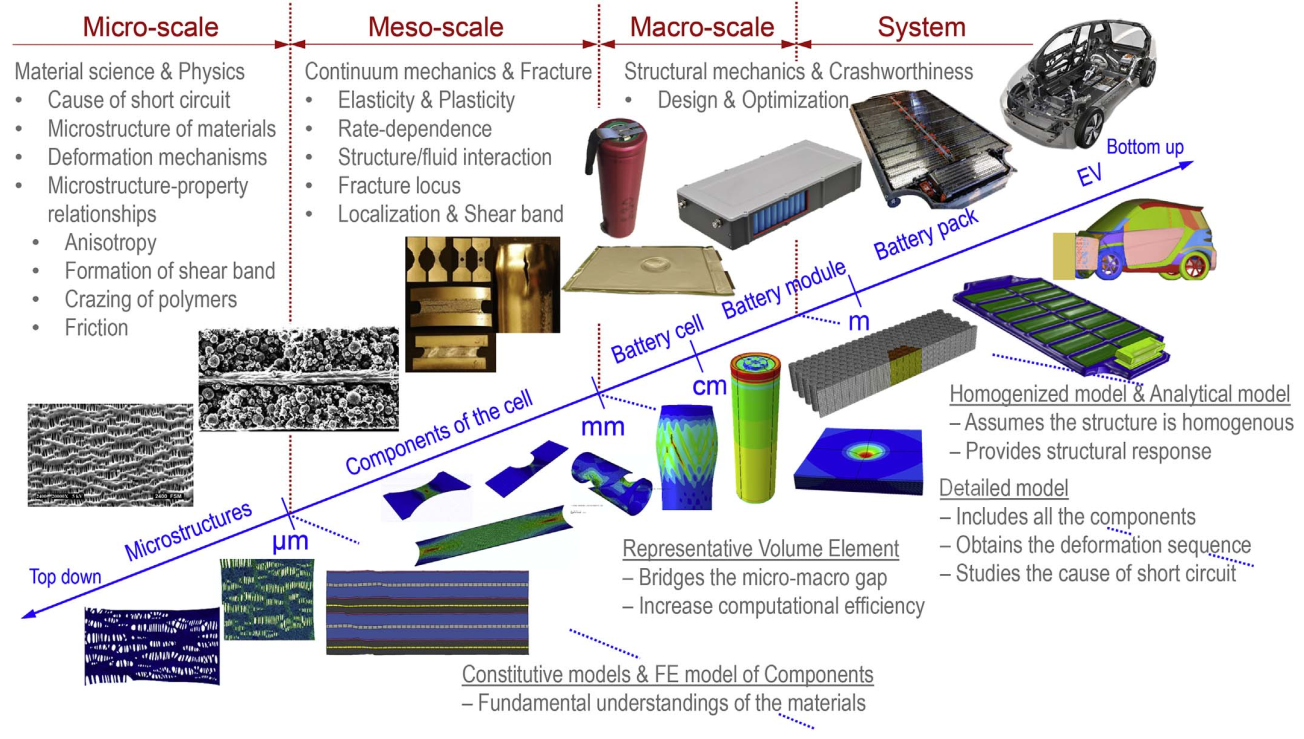
\includegraphics[width=0.8\linewidth]{zhu.png}
\caption{The study of mechanical properties of LIBs involves multiple scales and various models have been proposed to characterize the mechanical behavior of LIBs at each
length scale\cite{Zhu2018A}.}
\end{figure}

%----------------------------------------------------------------------------------------

\end{column} % End of the first column

\begin{column}{\sepwid}\end{column} % Empty spacer column

\begin{column}{\twocolwid} % Begin a column which is two columns wide (column 2)

\begin{columns}[t,totalwidth=\twocolwid] % Split up the two columns wide column

\begin{column}{\onecolwid}\vspace{-.6in} % The first column within column 2 (column 2.1)

%----------------------------------------------------------------------------------------
%	MATERIALS
%----------------------------------------------------------------------------------------

\begin{block}{Experiments Design}
The Specimen for testing of adhesion strength of Anode/Cathode and the loading method in different directions are shown as follows:
\begin{figure}
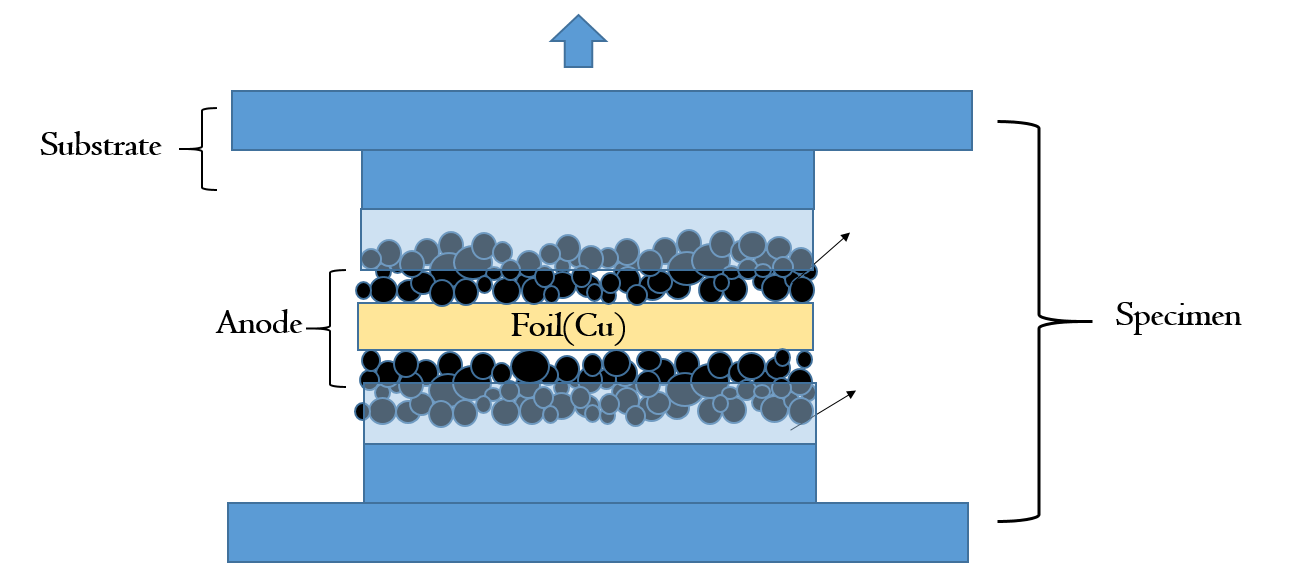
\includegraphics[width=\linewidth]{Specimen.png}
\caption{Specimen Preparation}
\end{figure}
\begin{figure}
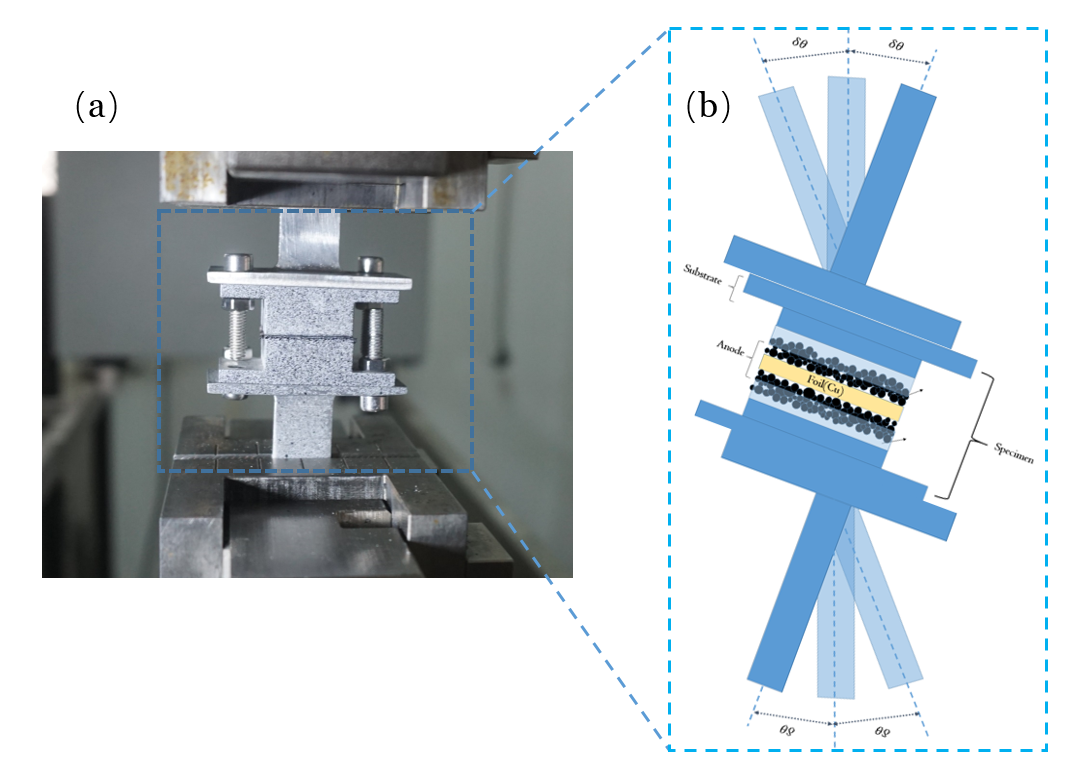
\includegraphics[width=\linewidth]{combine.png}
\caption{Combined Loading testways}
\end{figure}

\end{block}

%----------------------------------------------------------------------------------------

\end{column} % End of column 2.1

\begin{column}{\onecolwid}\vspace{-.6in} % The second column within column 2 (column 2.2)

%----------------------------------------------------------------------------------------
%	METHODS
%----------------------------------------------------------------------------------------

\begin{block}{Molecular Simulation Methods}
To study the change of mechanical properties of LiFePO4 during the Li-ion diffusion process(namely, in different SOCs), first principles density functional theory (DFT) calculations are adopted to calulate the energy barrier in B/C diffussion directions and the elastic constants(also the Young's modulus). \\
Based on the former simulation, the structures in the diffusion process can be established. So Molecular Dynamics Simulations are employed to study the stress-strain response of LiFePO4 in different SOCs under tensile and compression loading.\\
DFT calculations are conducted via Vienna ab initio simulation package\cite{Kresse1996Efficient}(VASP), and the Molecular Dynamics Simulations are conducted using LAMMPS\cite{Plimpton1995Fast}.
\end{block}

%----------------------------------------------------------------------------------------

\end{column} % End of column 2.2

\end{columns} % End of the split of column 2 - any content after this will now take up 2 columns width

%----------------------------------------------------------------------------------------
%	IMPORTANT RESULT
%----------------------------------------------------------------------------------------
\setbeamercolor{block alerted title}{fg=black,bg=norange} % Change the alert block title colors
\setbeamercolor{block alerted body}{fg=black,bg=white} % Change the alert block body colors 
\begin{alertblock}{Important Results}
For the \textbf{cathode}, the \textbf{shear strength} of
the coating-foil interface is almost \textbf{two times} of its \textbf{tensile
strength}. 
\textbf{Young's modulus} will have a \textbf{reduction of up to 23\%} during Li-ion diffusion. And \textbf{the intercalation of Li-ion reduces the fracture strain.}
\end{alertblock} 
%\begin{alertblock}{Important Result}

%Lorem ipsum dolor \textbf{sit amet}, consectetur adipiscing elit. Sed commodo molestie porta. Sed ultrices scelerisque sapien ac commodo. Donec ut volutpat elit.

%\end{alertblock} 

%----------------------------------------------------------------------------------------

\begin{columns}[t,totalwidth=\twocolwid] % Split up the two columns wide column again

\begin{column}{\onecolwid} % The first column within column 2 (column 2.1)

%----------------------------------------------------------------------------------------
%	MATHEMATICAL SECTION
%----------------------------------------------------------------------------------------

\begin{block}{Adhesion Strength Results}
The testing results of adhesion strength are shown:
\begin{figure}
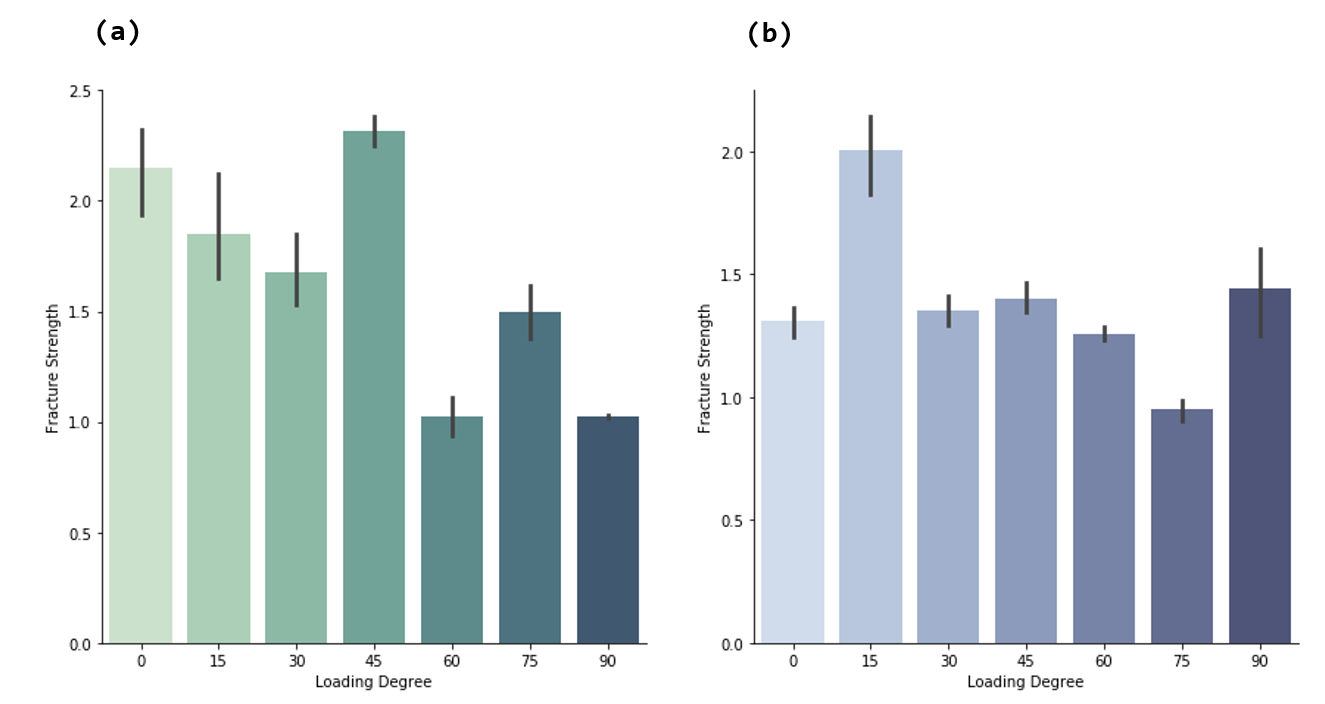
\includegraphics[width=\linewidth]{Strength.png}
\caption{Loading in different directions:(a)Cathode (b)Anode}
\end{figure}
Cohesive zone model is adopted for the tensile and shear component of anode:
\begin{figure}
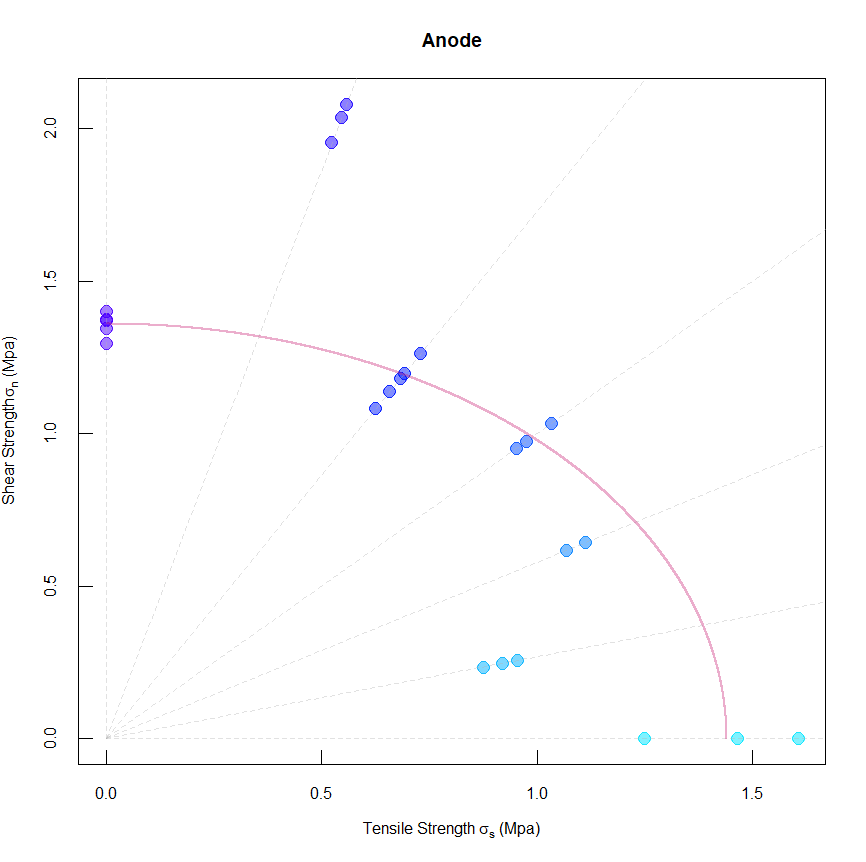
\includegraphics[width=0.8\linewidth]{circle.png}
%\caption{Cohesive Zone Model: Anode}
\end{figure}


\end{block}

%----------------------------------------------------------------------------------------

\end{column} % End of column 2.1

\begin{column}{\onecolwid} % The second column within column 2 (column 2.2)

%----------------------------------------------------------------------------------------
%	RESULTS
%----------------------------------------------------------------------------------------

\begin{block}{Molecular Simulation Results}
The energy barrier of Li-ion diffusion in B/C direction is shown:
\begin{table}
	\centering
    \begin{tabular}{ | c | c | c | }
    \hline
    \hline
    Direction & Barrier(eV) & $k_{HTST}$\\ \hline \hline
    B & 0.03 & $2.5 \times 10^6$\\
    C & 2.5 & $1.9 \times 10^{-26}$ \\
    \hline
    \hline
    \end{tabular}
\end{table}
And also the modulus during diffusion:\\
\begin{figure}
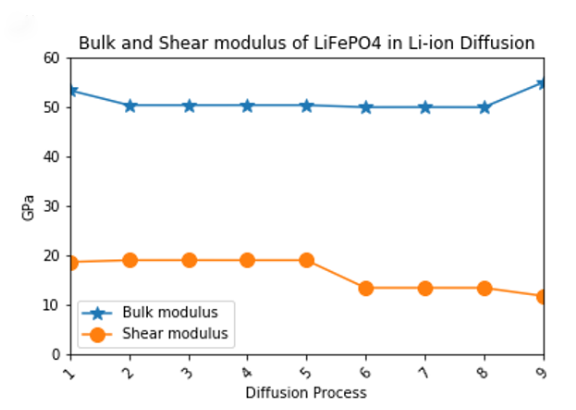
\includegraphics[width=0.8\linewidth]{modulus.png}
%\caption{The modulus changes during diffusion}
\end{figure}
The stress-strain response of LiFePO4 crystal and its fracture is shown below:
\begin{figure}
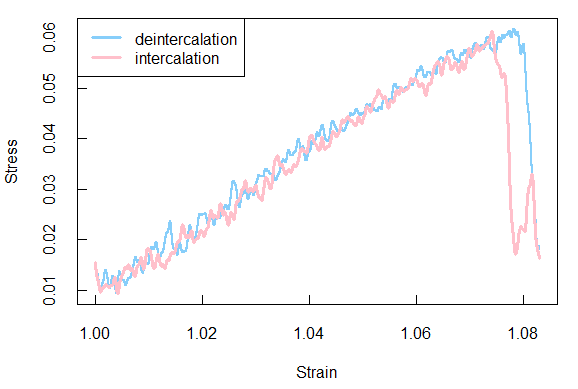
\includegraphics[width=0.9\linewidth]{md.png}
%\caption{The modulus changes during diffusion}
\end{figure}

\end{block}

%----------------------------------------------------------------------------------------

\end{column} % End of column 2.2

\end{columns} % End of the split of column 2

\end{column} % End of the second column

\begin{column}{\sepwid}\end{column} % Empty spacer column

\begin{column}{\onecolwid} % The third column

%----------------------------------------------------------------------------------------
%	CONCLUSION
%----------------------------------------------------------------------------------------

\begin{block}{Conclusion}
\begin{enumerate}
	\item The coating adhesion strength of anode and cathode varies between 0.9MPa and 2.4MPa and the strength of cathode is bigger than that of anode.
	\item \textbf{A combined adhesion and cohesion failure mode} was observed at the failure interface, where with larger shear component, the adhesion failure became dominant. 
	\item The mechanical properties(for example, Young's Modulus) can produce significant changes during the Li-ion diffusion process and \textbf{the fracture} will happen even for \textbf{perfect lattices} with the strain of about 7\%, and \textbf{the intercalation of Li-ion reduces the fracture strain.} 
\end{enumerate}
\end{block}



%----------------------------------------------------------------------------------------
%	ADDITIONAL INFORMATION
%----------------------------------------------------------------------------------------

%----------------------------------------------------------------------------------------
%	REFERENCES
%----------------------------------------------------------------------------------------

\begin{block}{References}

\nocite{*} % Insert publications even if they are not cited in the poster
\small{\bibliographystyle{plain}
\bibliography{sample}\vspace{0.75in}}

\end{block}

%----------------------------------------------------------------------------------------
%	ACKNOWLEDGEMENTS
%----------------------------------------------------------------------------------------



\begin{block}{Acknowledgements}

\small{\rmfamily{I would like to thank my advisor, Prof. Xia Yong, for his continuous guidance and support through the whole research. I am grateful to my committee members, Prof. Zhou Qing and Phd Pan Zhexin for their constructive comments. }} \\
\end{block}

%----------------------------------------------------------------------------------------
%	CONTACT INFORMATION
%----------------------------------------------------------------------------------------

%\setbeamercolor{block alerted title}{fg=black,bg=norange} % Change the alert block title colors
%\setbeamercolor{block alerted body}{fg=black,bg=white} % Change the alert block body colors

\begin{alertblock}{Contact Information}

\begin{itemize}
\item Web: \href{http://resume.feiyuxiao.xyz/}{http://resume.feiyuxiao.xyz}
\item Email: \href{feiyuxiaothu@gmail.com}{feiyuxiaothu@gmail.com}
\end{itemize}

\end{alertblock}

\begin{center}
\begin{tabular}{ccc}

\includegraphics[width=0.5\linewidth]{logo.png} & \hfill & 
\includegraphics[width=0.5\linewidth]{Tsinghua.png}
\end{tabular}
\end{center}

%----------------------------------------------------------------------------------------

\end{column} % End of the third column

\end{columns} % End of all the columns in the poster

\end{frame} % End of the enclosing frame

\end{document}
